\lesson{3}{6 February 2025 9:00}{Chapter 1}

\begin{definition}[Globalization]
    The process whereby national or regional 
    economies and cultures have become integrated through:
    \begin{itemize}
        \item New global communication technologies.
        \item Foreign direct investment.
        \item International trade.
        \item Migration.
        \item New forms of transportation.
        \item Flow of money.
    \end{itemize}
\end{definition}

\subsection{History of Globalization (not on test)}
\begin{itemize}
    \item Began after WWII with the establishment of the United Nations and fostering of trade relations between countries.
    \item Economic ties between countries strengthened -- tax treaties were negotiated, tariffs abolished, global corporations developed
    \item New technology allows international business to occur in real time, transforming the globe into one market.
    \item Has increased interdependence of all nations, blurring political boundaries
\end{itemize}

\begin{definition}[Interdependence]
    The reliance of two or more nations on each other for products or services.
\end{definition}

\textbf{Three Main Areas of Interdependence:}
\begin{itemize}
    \item Primary industries
    \item Secondary industries 
    \item Tertiary industries
\end{itemize}

\begin{definition}[Multiplier Effect]
    When an entity (such as the government, businesses, or individuals) spends money, it generates income for others, who in turn spend that income, creating a ripple effect through the economy.
\end{definition}

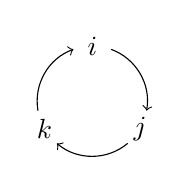
\begin{tikzpicture}[->,scale=.7]
   \node (i) at (90:1cm)  {$i$};
   \node (j) at (-30:1cm) {$j$};
   \node (k) at (210:1cm) {$k$};
%   \node (l) at () {$l};
%   \node (m) at () {$m};

   \draw (70:1cm)  arc (70:-10:1cm);
   \draw (-50:1cm) arc (-50:-130:1cm);
   \draw (190:1cm) arc (190:110:1cm);
\end{tikzpicture}